\chapter{پیاده‌سازی}

در بخش قبلی معماري کلی سامانه و ماژول‌هاي موردنیاز براي پیاده سازي سامانه پایش شبکه را بیان و به صورت اجمالی معرفی کردیم. در این فصل به چگونگی قرار گرفتن و ارتباط بخش‌هاي مختلف می‌پردازیم و پیاده سازي سیستم را توضیح خواهیم داد.


ماژول‌های تعریف شده در فصل قبل برای سامانه پایش شبکه‌های کامپیوتری را می‌توان در چهار دسته کلی قرار داد: 

\begin{itemize}
    \item هسته \lr{SNMP}
    \item فرانت‌اند 
    \item بک‌اند
    \item ذخیره‌سازی اطلاعات


\end{itemize}

در ادامه برای هر دسته توضیحاتی ارائه خواهد شد. این توضیحات شامل ماژول‌های دربرگیرنده آن، بررسی راه‌های ممکن برای پیاده سازی هر ماژول و درنهایت نحوه پیاده سازی آن ماژول خواهد بود. 


\section{هسته \lr{SNMP}}

این دسته فقط شامل ماژول هسته \lr{SNMP} از \cref{fig.11} است. برای این ماژول هدف، توسعه ابزاری است که بتوان از طریق آن انواع پیام‌های \lr{SNMP} را ارسال و دریافت کرد. بدین منظور با تعریف دو کلاس \lr{Trap} و \lr{Session} این ماژول را پیاده سازی می‌کنیم. توجه شود که کتابخانه \lr{net-snmp} به زبان \lr{C} است ولی این ماژول جهت توسعه بهینه در زبان \lr{C++} توسعه داده شد. در نهایت ابزاری برای این ماژول تولید شد که قابلیت دریافت پیام‌های \lr{Trap} از طریق کلاس \lr{Trap} و همچنین  ارسال و دریافت \lr{get} و \lr{walk} از طریق کلاس \lr{ Session } را دارد.

\newpage

\section{فرانت‌اند}

این دسته فقط شامل ماژول رابط کاربری تحت وب از \cref{fig.11} است. این قسمت برای توسعه بهینه همانطور که در فصل قبل گفته شد با فریمورک ری‌اکت توسعه داده شد. در این قسمت قدم به قدم رابط کاربری توسعه داده شده به همراه کارایی آن مورد بررسی قرار می‌دهیم.


در \cref{fig.12} و \cref{fig.13} منو‌های سامانه نشان داده می‌شود که شرح مختصری از آن‌ها در ادامه آورده شده است:


\begin{figure}[!h]
    \centering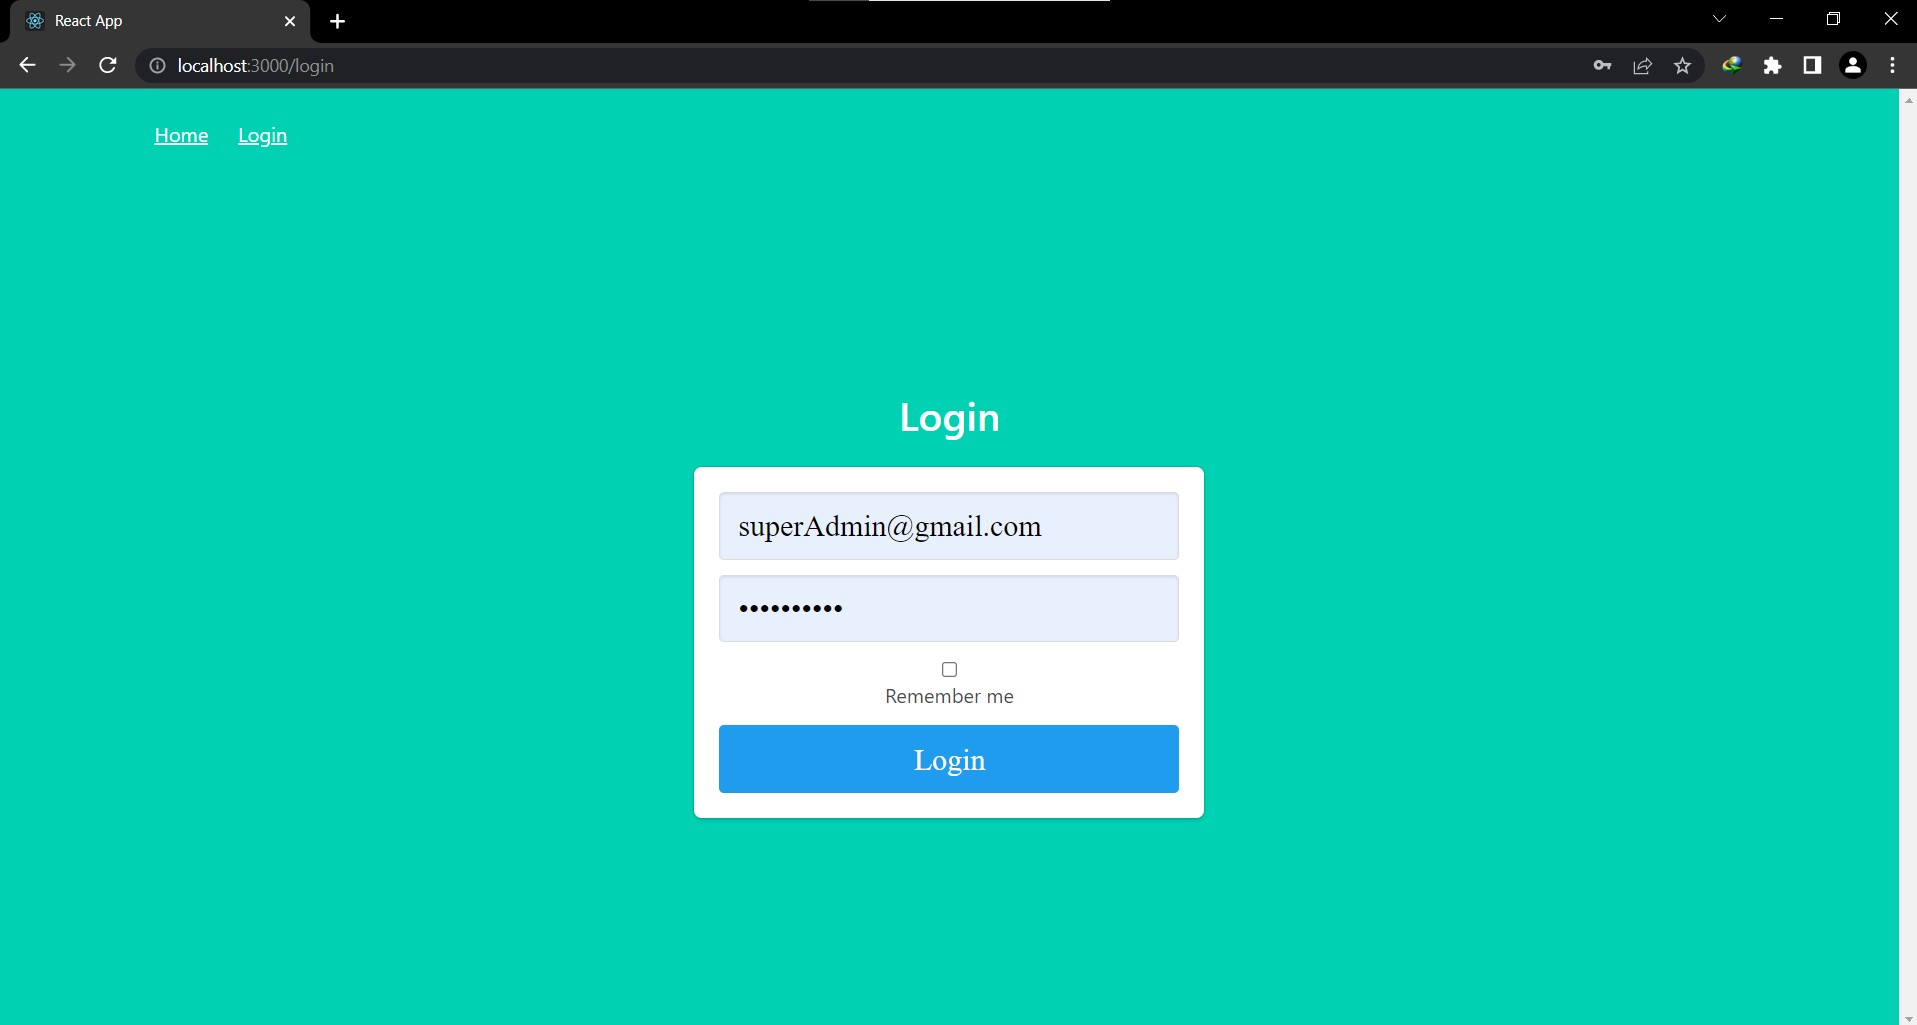
\includegraphics[scale=.38]{./nav-logout}
    \caption{منوی سیستم هنگام لاگین}\label{fig.12}
\end{figure}

\begin{figure}[!h]
    \centering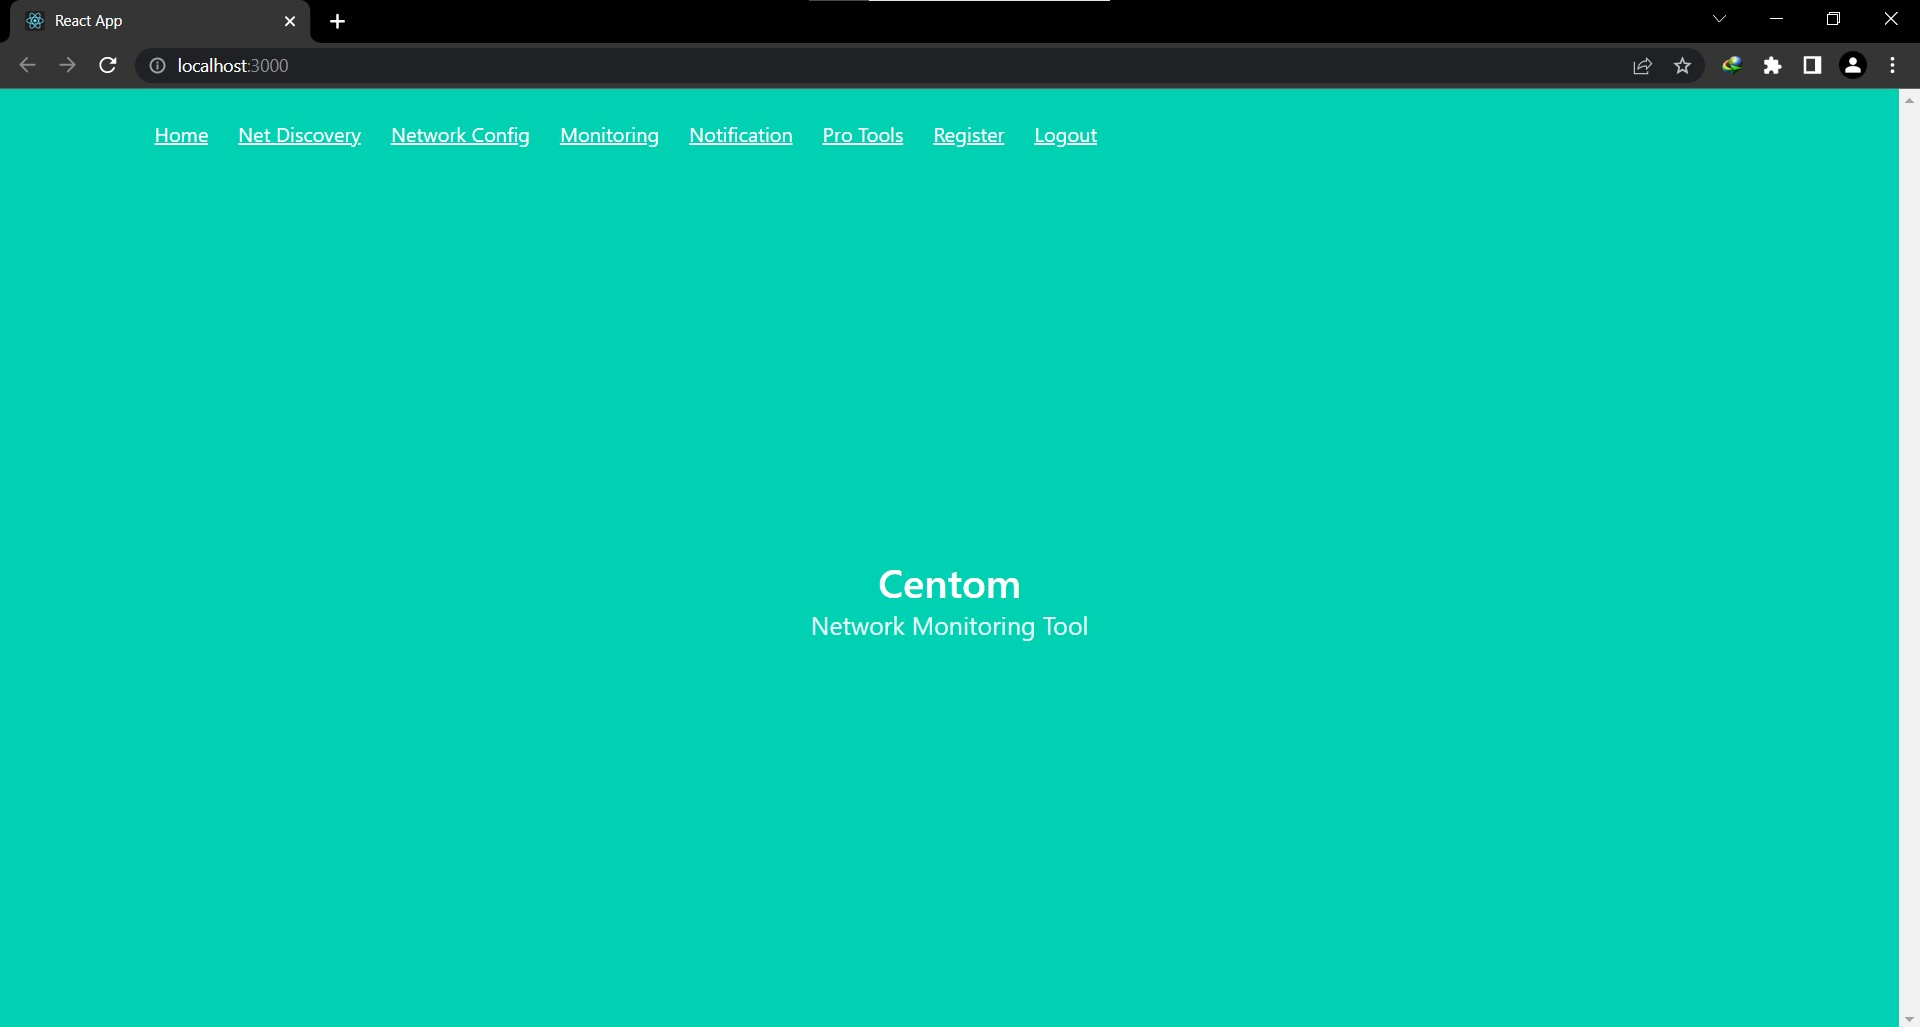
\includegraphics[scale=.38]{./nav-login}
    \caption{منوی سیستم بعد از لاگین ادمین ارشد}\label{fig.13}
\end{figure}
        
زمانی که کاربری لاگین نکرده است(\cref{fig.12})، تنها دو صفحه خانه و لاگین قابل دسترسی خواهد بود. این بدان علت است که در این سامانه ثبت نام کاربر فقط توسط ادمین ارشد صورت می‌گیرد. در \cref{fig.13} منوها پس از لاگین ادمین ارشد نمایش داده شده‌اند. تاکیر بر روی ادمین ارشد بدین علت است که در این سامانه سه سطح دسترسی ادمین ارشد، ادمین معمولی و کاربر عادی وجود دارد. ادمین ارشد به همه امکانات، ادمین معمولی به ثبت نام کاربر جدید، تنظیمات و اسکن شبکه دسترسی ندارد. کاربر عادی نیز فقط به اسکن سریع یک دستگاه دسترسی خواهد داشت. البته این سامانه فقط یک ادمین ارشد خواهد داشت!

\newpage

تعریف کاربر جدید فقط توسط ادمین ارشد تحت رجیستر در \cref{fig.14} ممکن خواهد بود. برای ثبت نام یک کاربر، ادمین ارشد باید یک ایمیل، رمز عبور وارد نماید. سپس باید بین دو نقش ادمین معمولی ویا کاربر معمولی انتخاب نماید. در نهایت ایمیل و رمز عبور را در اختیار شخص متقاضی قرار می‌دهد.


\begin{figure}[!h]
    \centering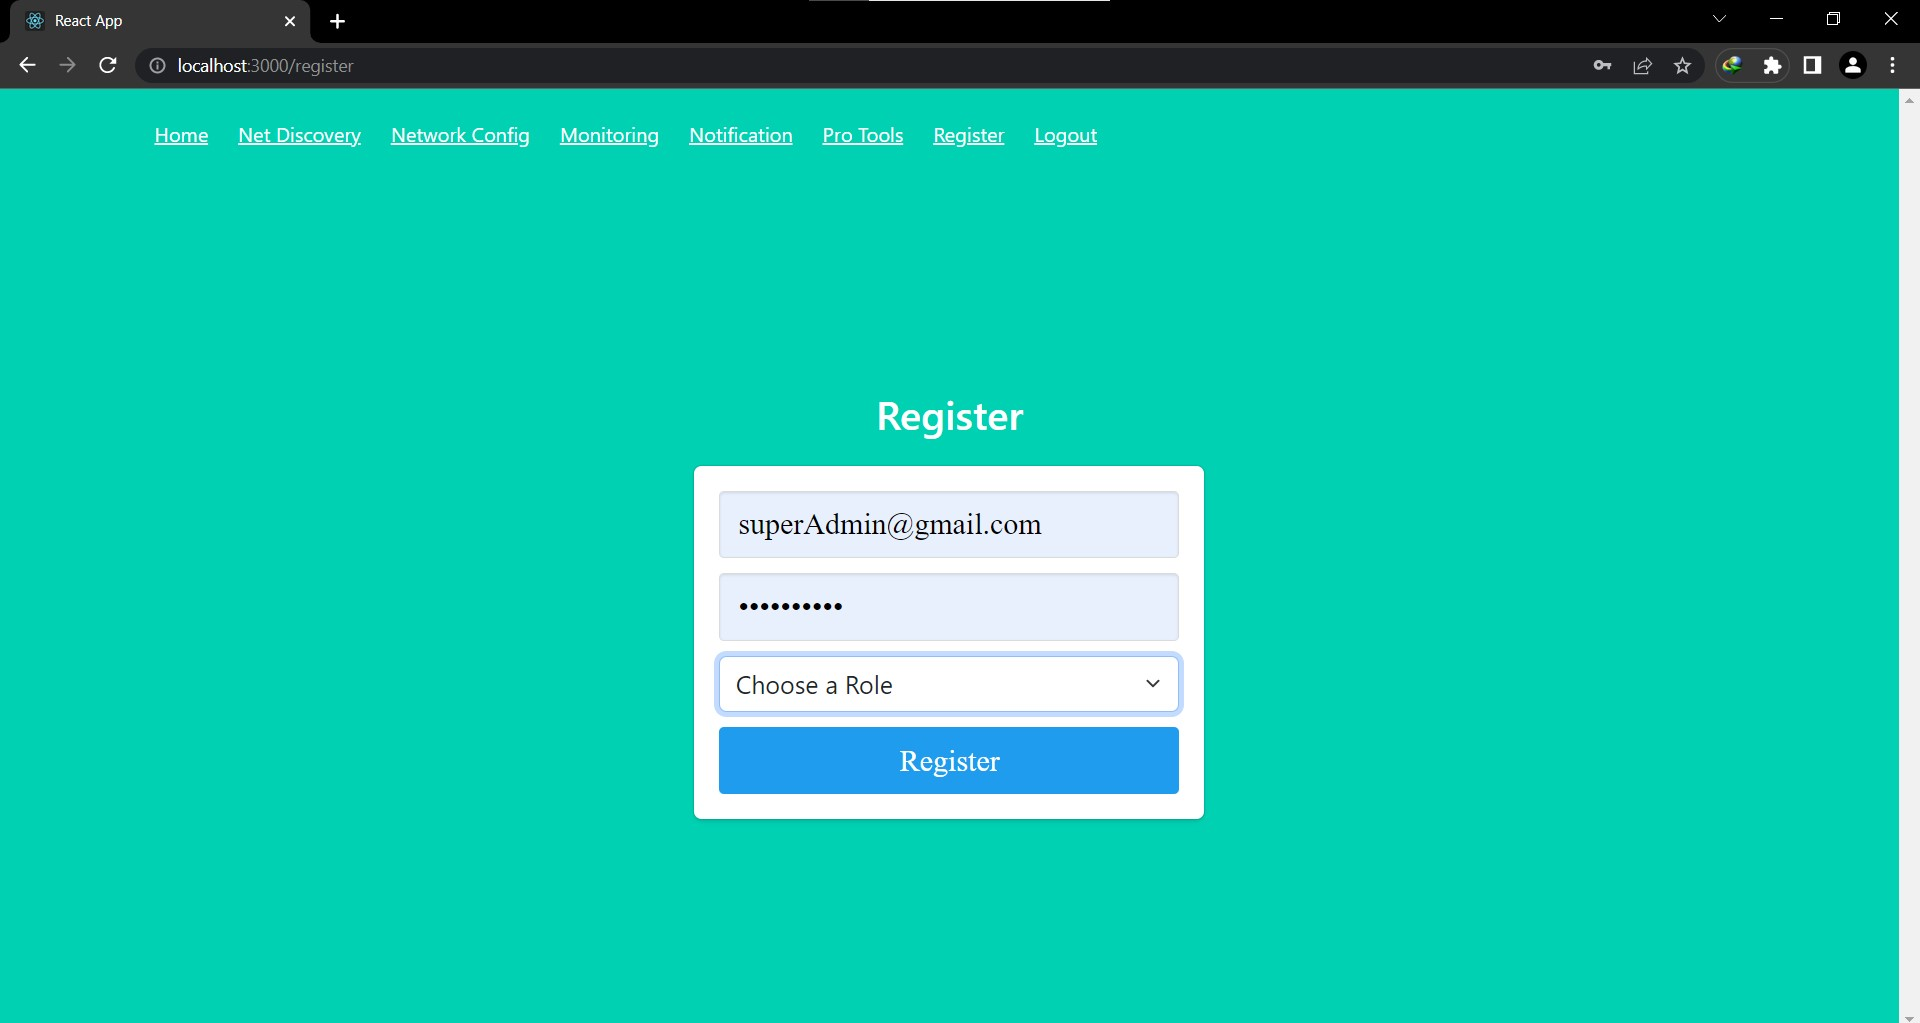
\includegraphics[scale=.38]{./register}
    \caption{صفحه رجیستر در اختیار ادمین ارشد}\label{fig.14}
\end{figure}


مهم‌ترین قسمت این سامانه، کشف شبکه است که اولین منو بعد از منوی خانه قرار دارد. رابط کاربری این قسمت قبل و بعد از تست در \cref{fig.15} و \cref{fig.16} نشان داده شده‌ است. 


\begin{figure}[!h]
    \centering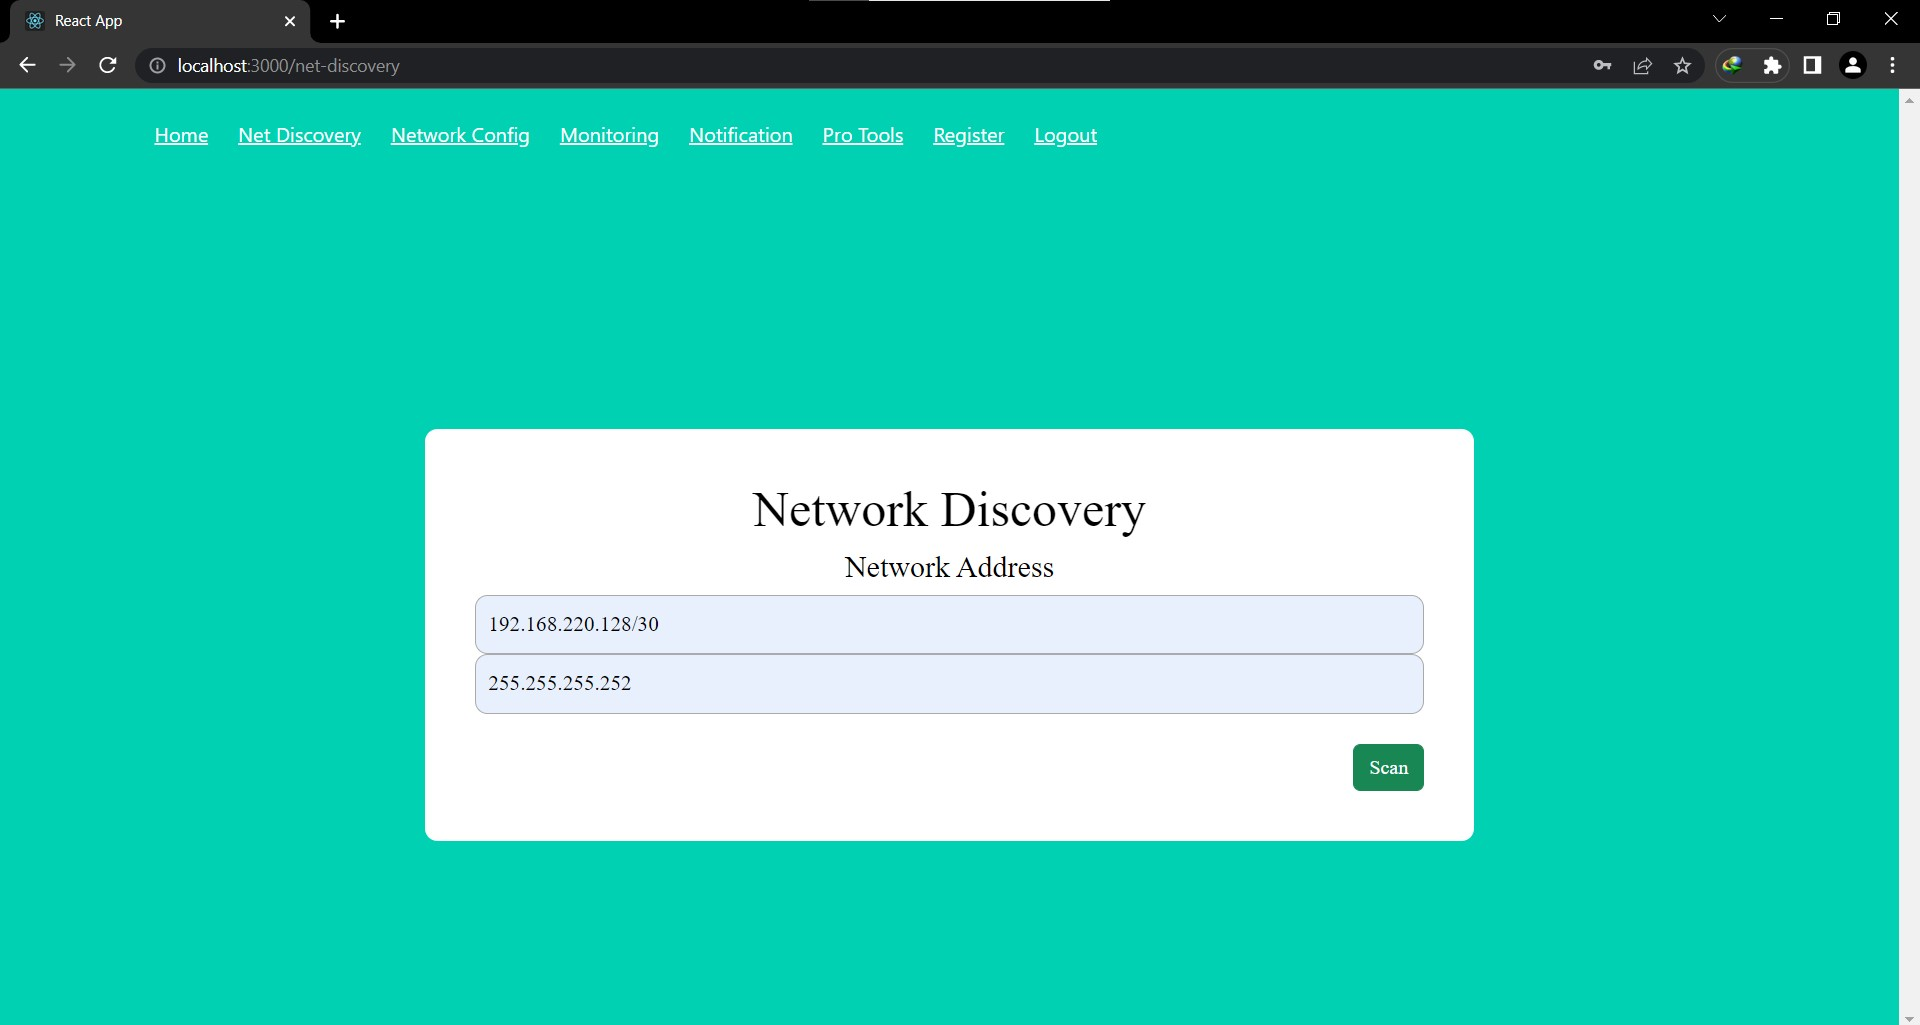
\includegraphics[scale=.38]{./net-dis-before}
    \caption{صفحه کشف شبکه قبل از اسکن}\label{fig.15}
\end{figure}


\begin{figure}[!h]
    \centering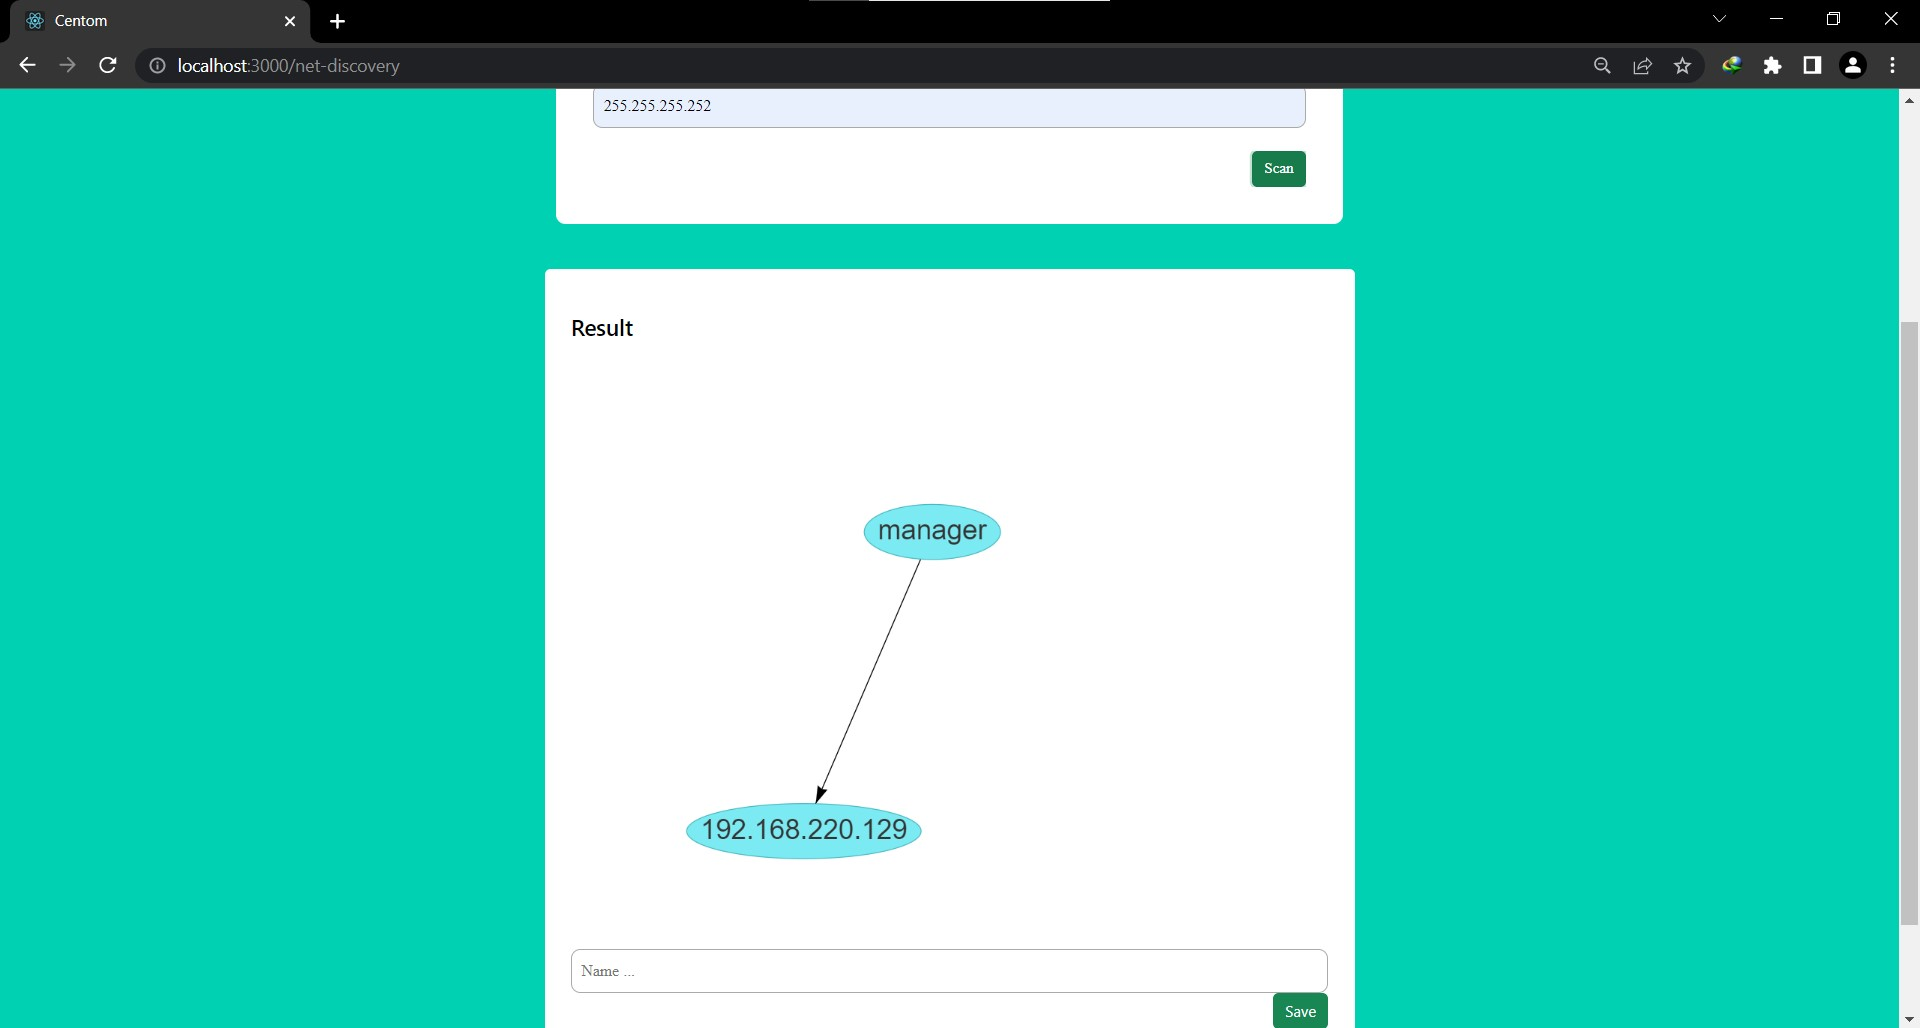
\includegraphics[scale=.38]{./net-dis-after}
    \caption{خروجی اسکن شبکه در قالب یک گراف}\label{fig.16}
\end{figure}


در کشف شبکه ابتدا یک آدرس شبکه به همراه \lr{Subnet Mask} از ادمین ارشد گرفته می‌شود. سپس بعد از اتمام اسکن شبکه، خروجی در قالب یک گراف نمایش داده می‌شود. درنهایت ادمین ارشد می‌تواند در صورت نیاز شبکه را با اسمی دلخواه در سامانه ذخیره کند.


بعد از ذخیره‌ سازی شبکه در قسمت قبل، ادمین ارشد می‌تواند ابتدا اطلاعات و تنظیمات شبکه را وارد نماید و بعد از آن اقدام به پایش شبکه کند. بدین ترتیب بعد از منوی کشف شبکه، منوی ذخیره تنظیمات شبکه در \cref{fig.17} وجود دارد. ابتدا با انتخاب اسم شبکه و نوع دستگاه‌های مورد نظر سامانه لیستی از آدرس‌ها را نشان می‌دهد. که با انتخاب یک آدرس مشخصات آن توسط کاربر وارد می‌شود. همچنین می‌تواند پارامترهای مورد نظر برای پایش دستگاه را به صورت لیست اضافه کند.



\begin{figure}[!h]
    \centering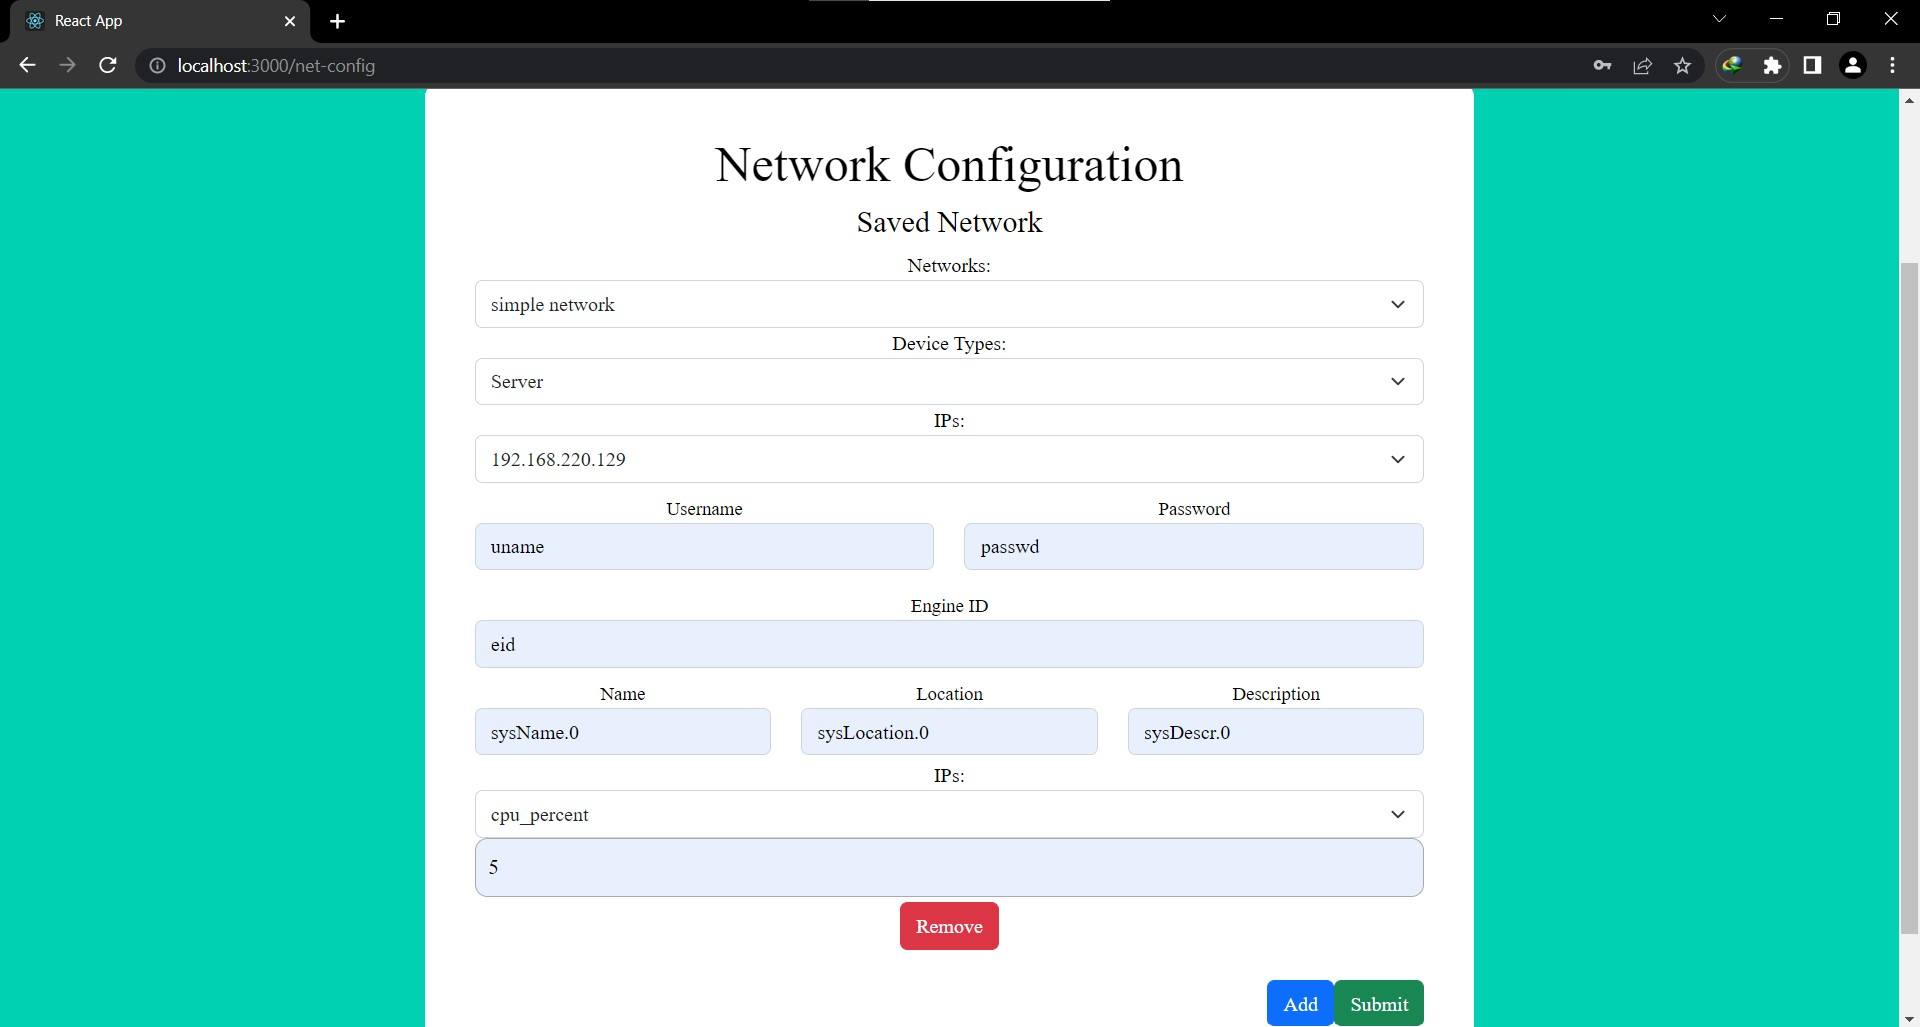
\includegraphics[scale=.38]{./net-config}
    \caption{صفحه ذخیره تنظیمات شبکه}\label{fig.17}
\end{figure}





% مانیتورینگ ///////////////////////////////////////////////////////////////////////////////////////////////////////
% نوتیفیکیشن //////////////////////////////////////////////////////////////////////////////////////////////////////


در نهایت منوی ابزارهای پیشرفته قرار دارد، که در حال حاضر تنها اسکن سریع آن در \cref{fig.120} موجود است. سامانه در این قسمت می‌تواند با دریافت یک آدرس و یک شناسه شی، پیام‌های \lr{get} و \lr{walk} را ارسال و نتیجه را به ترتیب مشاهده کند. 

\begin{figure}[!h]
    \centering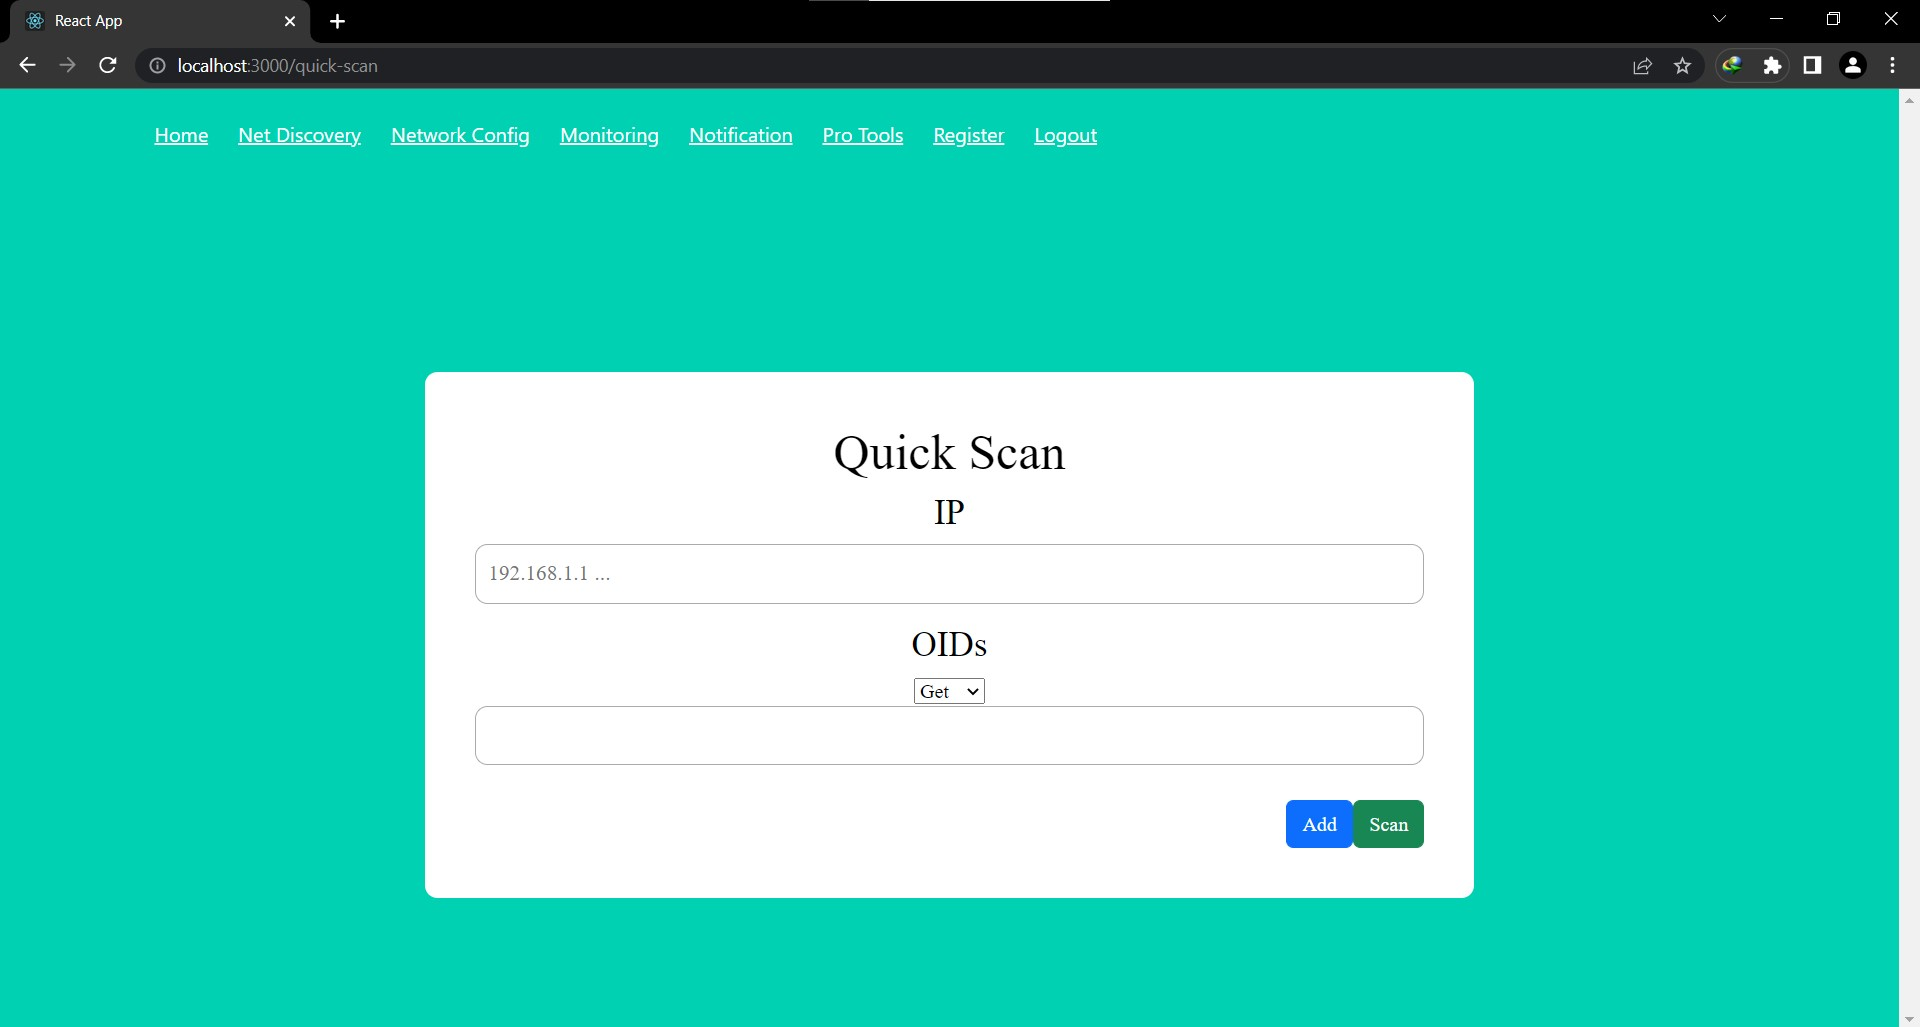
\includegraphics[scale=.38]{./pro-tools}
    \caption{صفحه ابزارهای پیشرفته}\label{fig.120}
\end{figure}




\section{ذخیره‌سازی اطلاعات}





\section{بک‌اند}





\section{خلاصه}
